\documentclass[twocolumn]{article}
\usepackage{float}
\usepackage{graphicx}
\usepackage{fancyhdr}
\usepackage{geometry}
\usepackage{xcolor, soul}
\usepackage{changepage}  % allows temporary margin adjustments
\usepackage{amsmath}
\usepackage[font=footnotesize, justification=centering]{caption}
\usepackage{subcaption}
\usepackage{wrapfig}
\usepackage{multirow}
\usepackage{booktabs}
\usepackage{amssymb}
\usepackage{soul,xcolor}
\usepackage{pgfplots}
\pgfplotsset{compat=1.18}
\usepackage{siunitx}
\usepackage{url}
\usepackage{ctable}
\usepackage{natbib}
\bibliographystyle{plain}
\usepackage{cleveref}
\usepackage{physics}
\usepackage[inline]{enumitem}
\usepackage{overpic}
\usepackage[normalem]{ulem}
\usetikzlibrary{intersections}
\usepgfplotslibrary{fillbetween}

\geometry{margin=2cm}

\setlength{\fboxsep}{0pt} % Padding between border and image
\setlength{\fboxrule}{0.5pt} % Thickness of the border

\title{\textbf{4A2 CFD Interim Report}}
\author{
  2266T
  \and
  \today\\}
\date{}

\begin{document}

\maketitle

\section{Results: bump and bend cases}

\subsection{Bump case}

\begin{figure}[H]
    \centering
    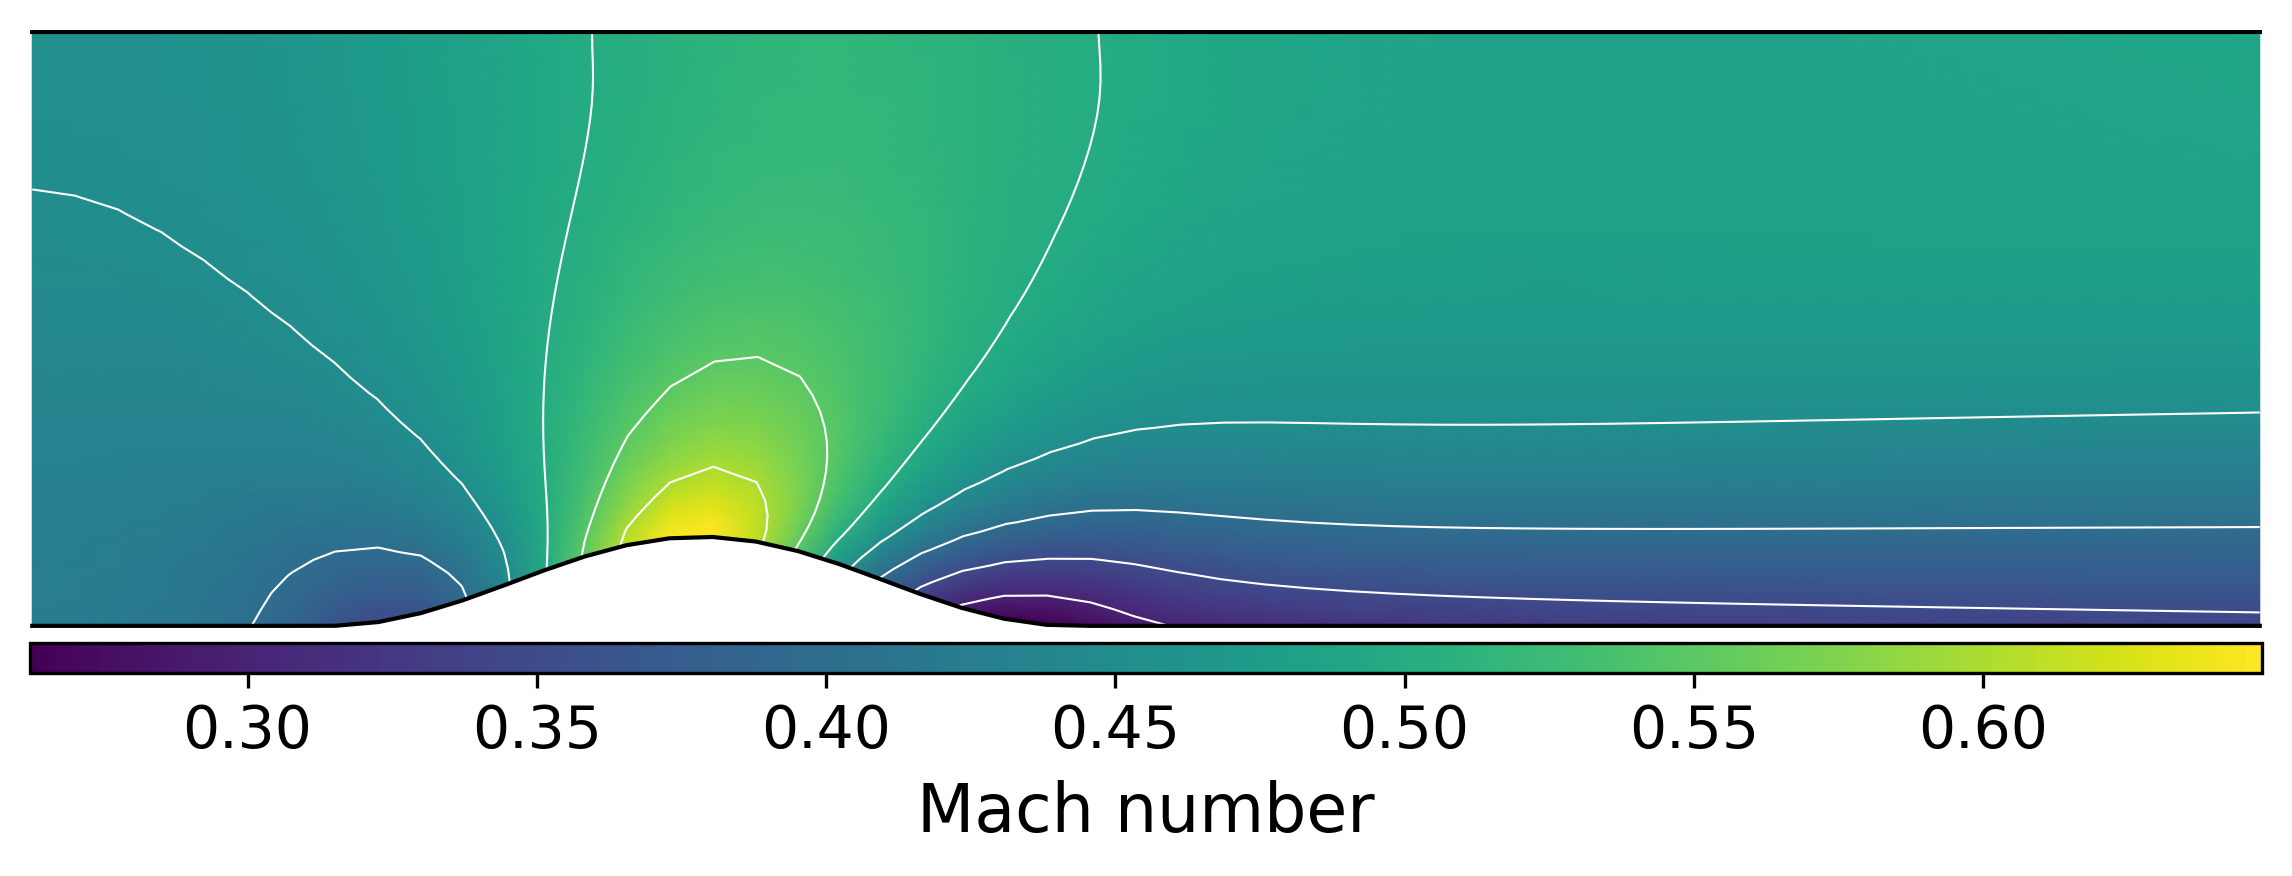
\includegraphics[width=\linewidth]{plots/contour_plots_bump_mach.png}
    \caption{Bump case Mach number results.}
    \label{fig:bump_mach}
\end{figure}

\begin{figure}[H]
    \centering
    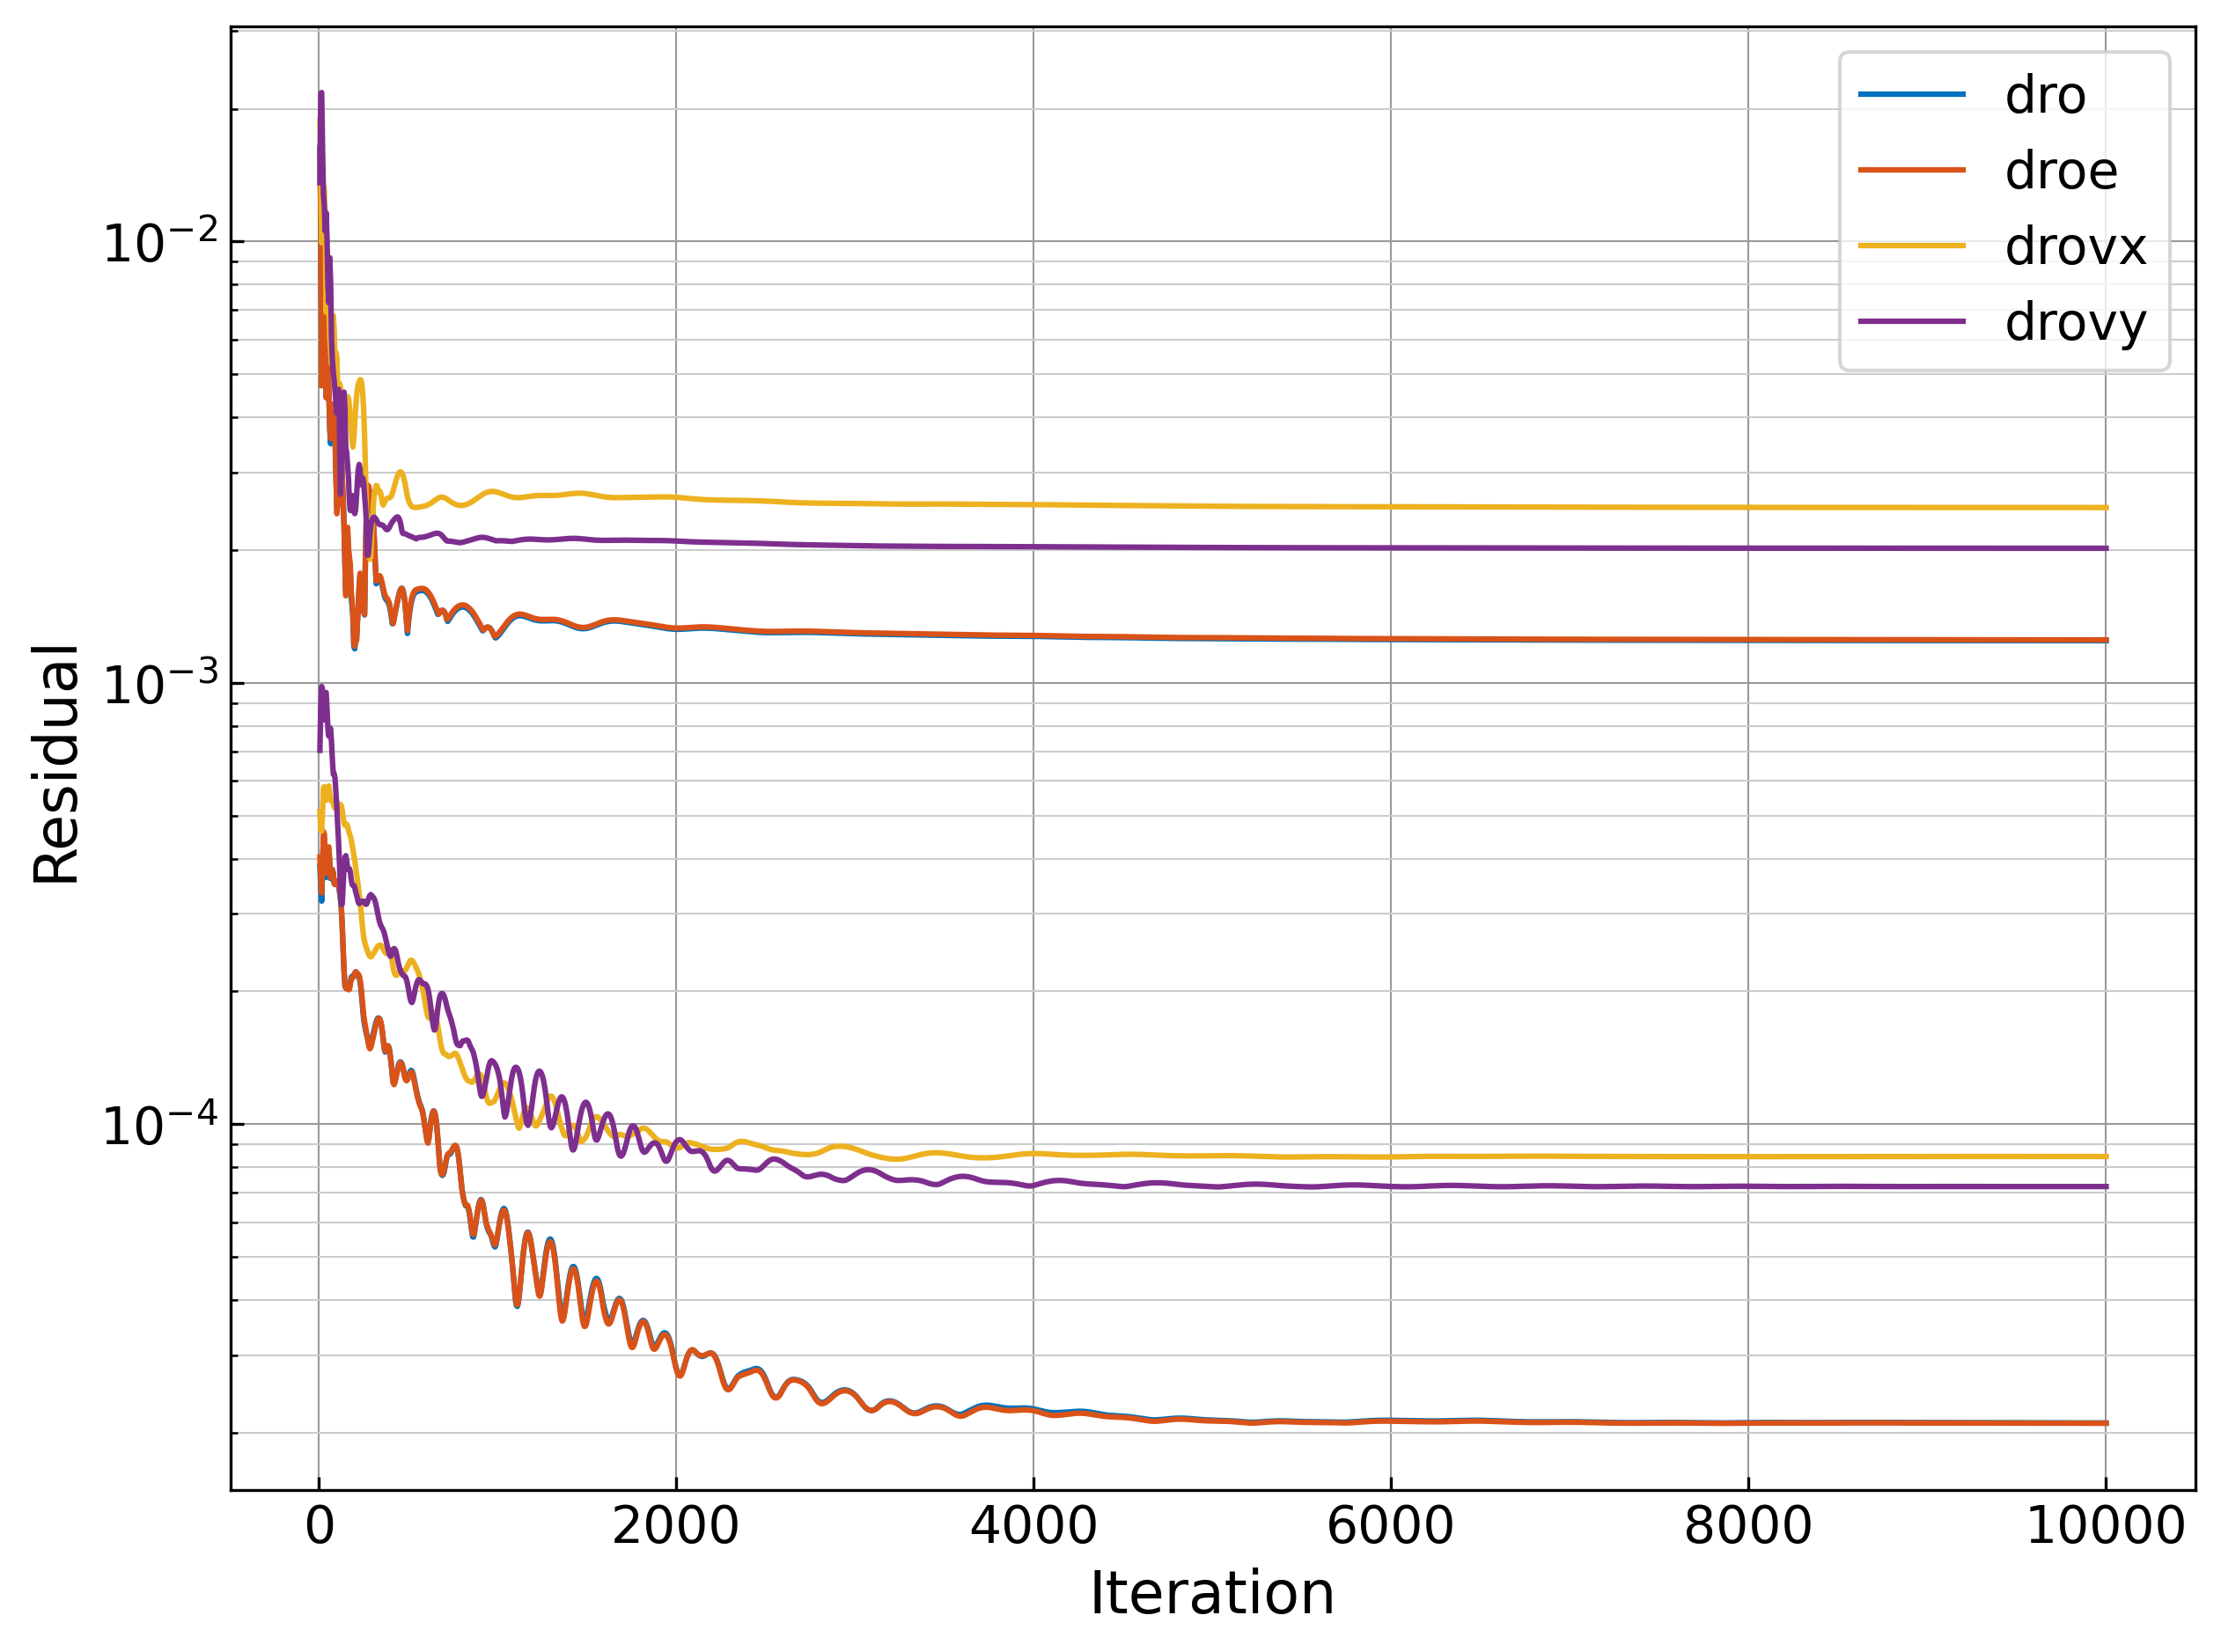
\includegraphics[width=\linewidth]{plots/convergence_plot_bump.png}
    \caption{Bump case convergence results.}
    \label{fig:bump_convergence}
\end{figure}

\subsection{Bend case}

\begin{figure}[H]
    \centering
    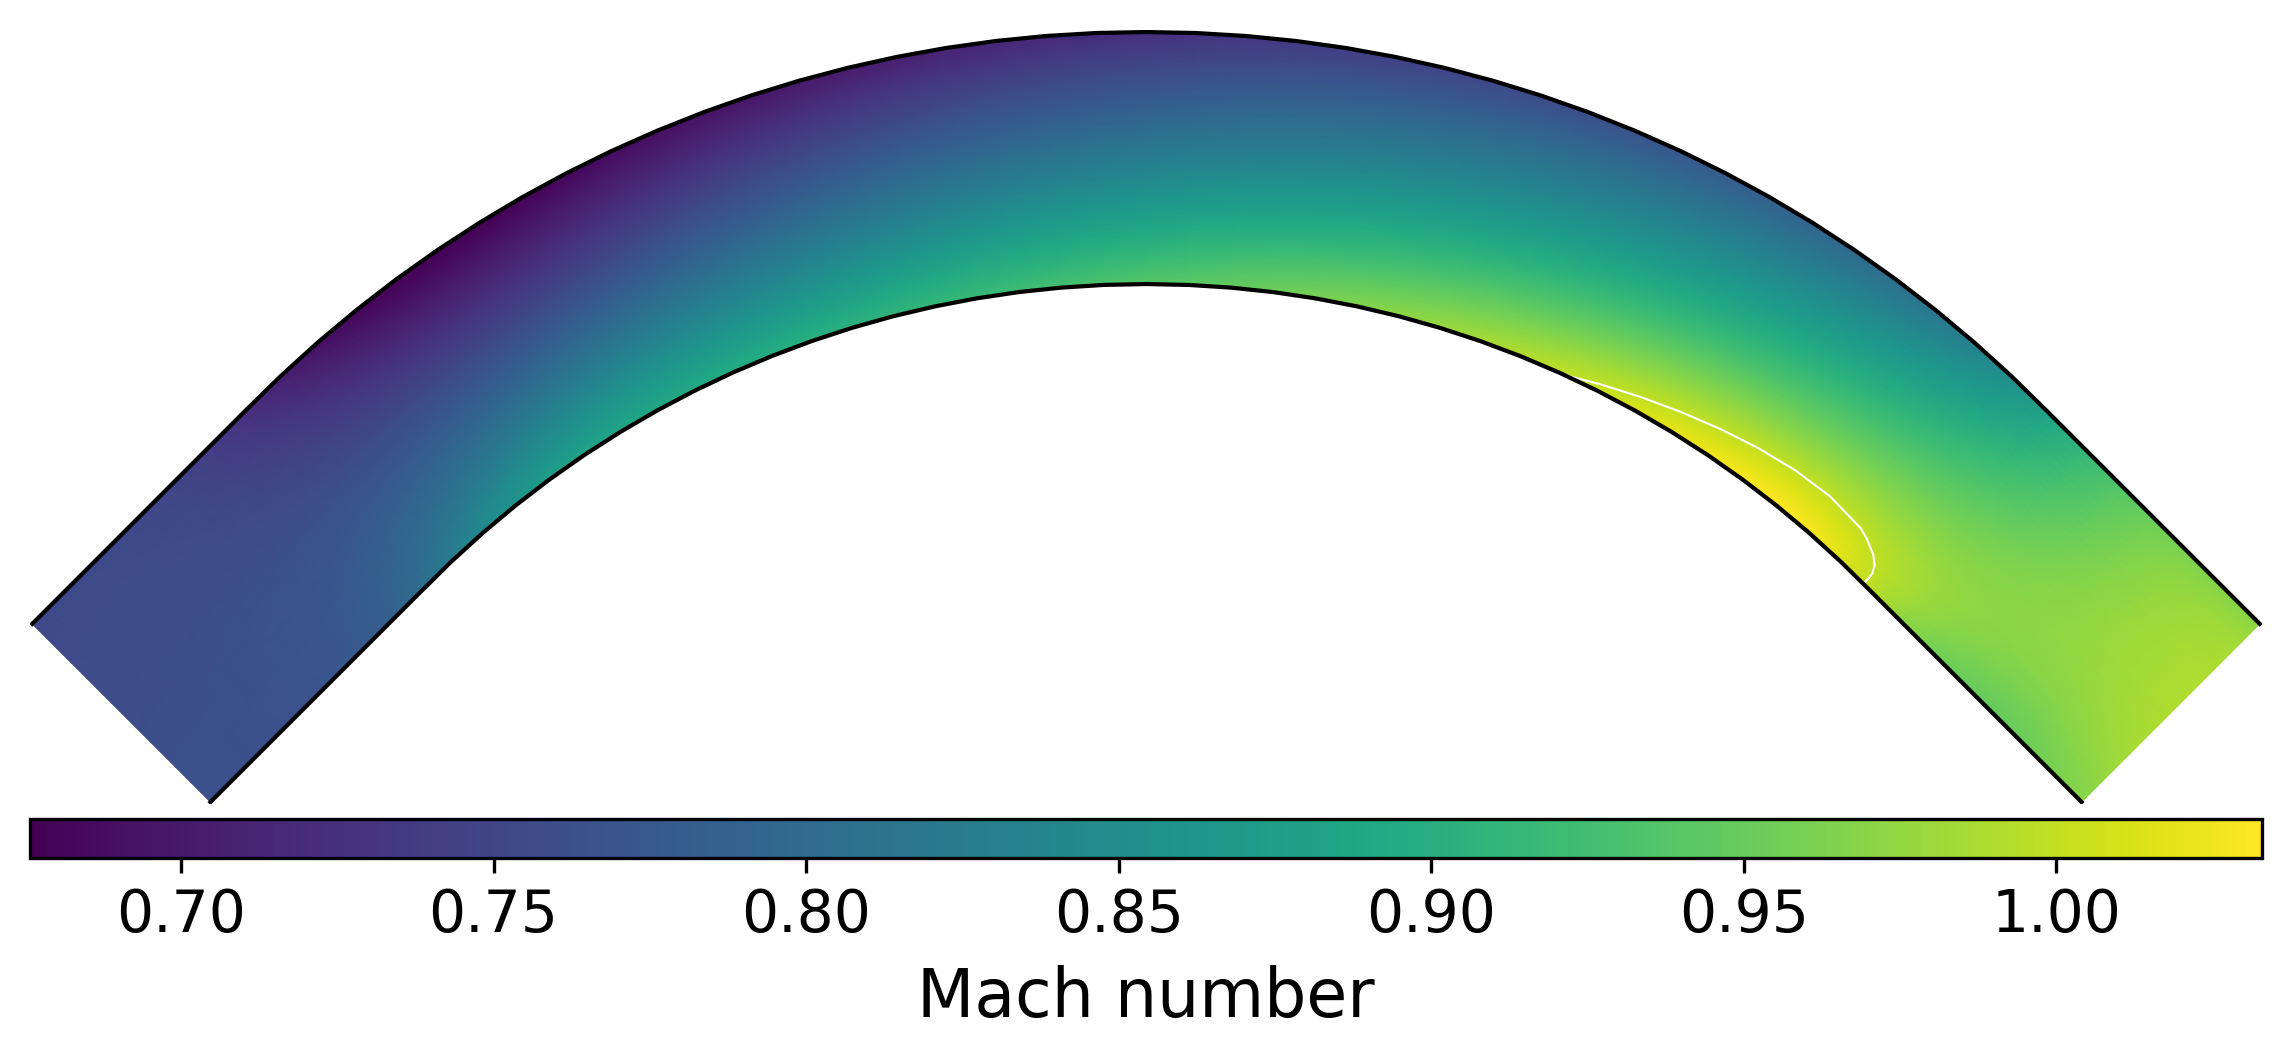
\includegraphics[width=\linewidth]{plots/contour_plots_bend_mach.png}
    \caption{Bend case Mach number results.}
    \label{fig:bend_mach}
\end{figure}

\begin{figure}[H]
    \centering
    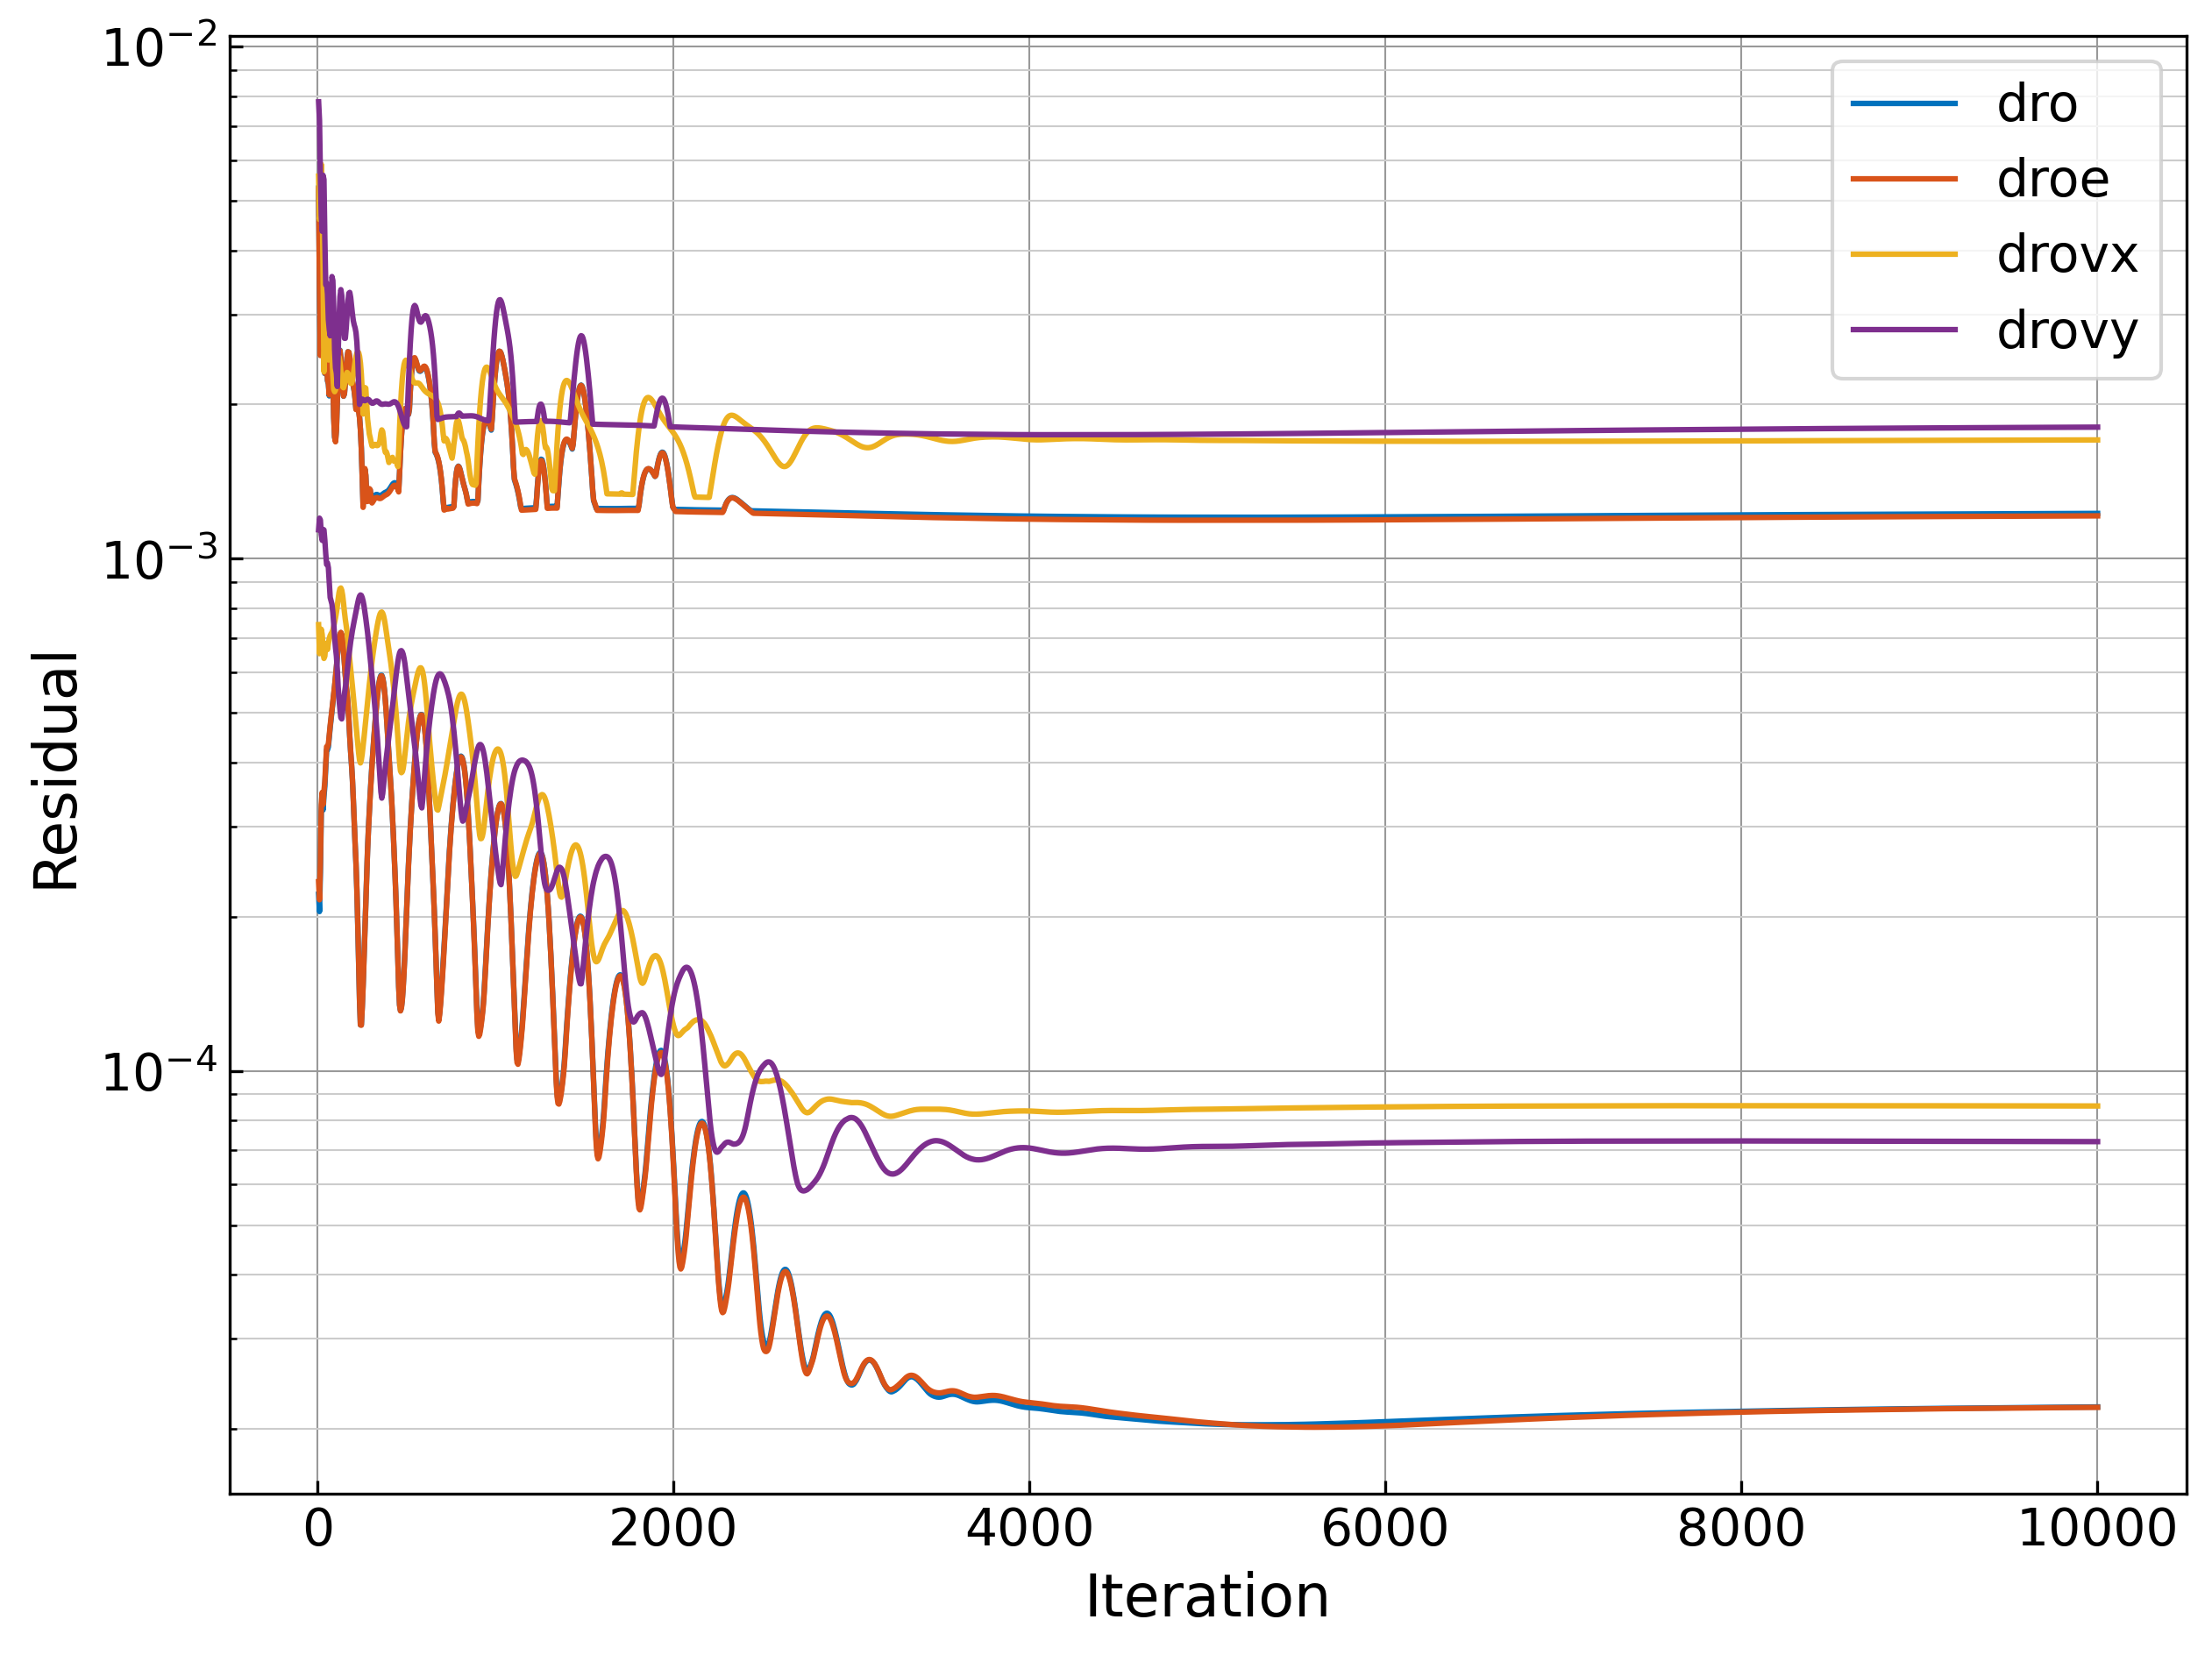
\includegraphics[width=\linewidth]{plots/convergence_plot_bend.png}
    \caption{Bend case convergence results.}
    \label{fig:bend_convergence}
\end{figure}

\section{Accuracy and parameter effects}
% Discuss accuracy, CFL number, smoothing factor, mesh size,
% stability, and runtime. Support the discussion with figures.

\subsection{Effects of varying CFL number}

\begin{figure}[H]
    \centering
    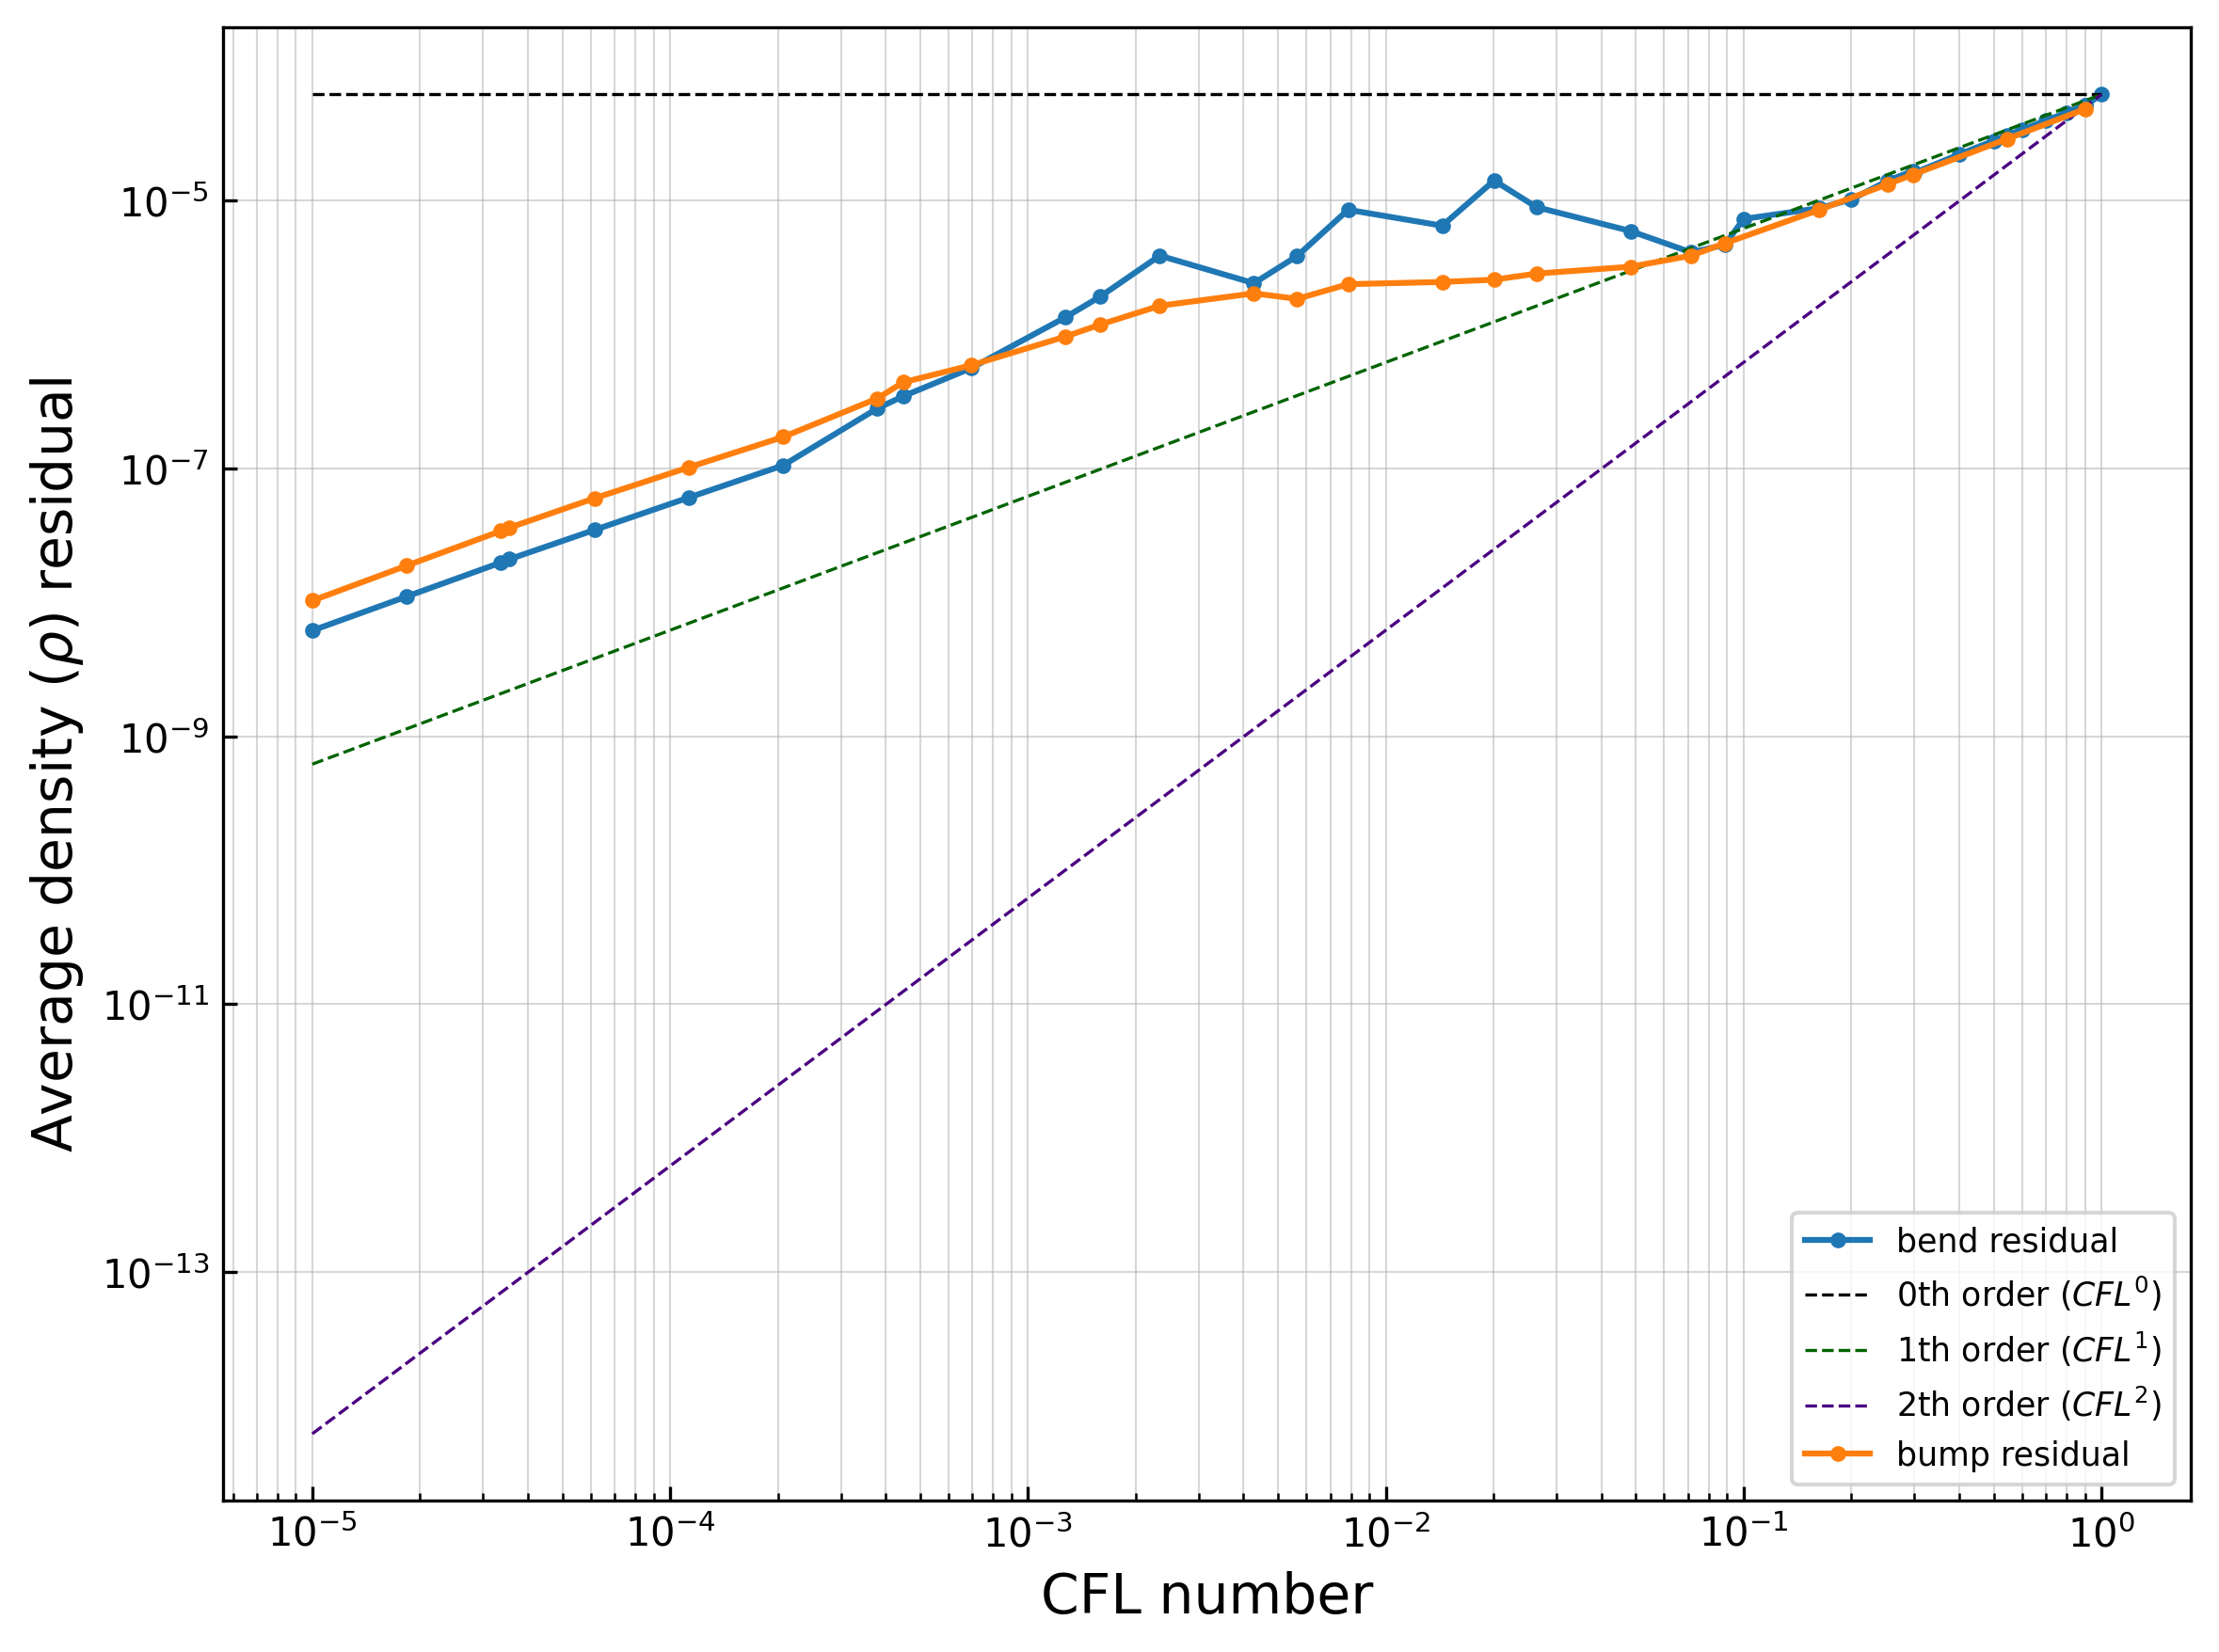
\includegraphics[width=\linewidth]{plots/convergence_plot_CFL.png}
    \caption{Convergence results of the bend and bump cases with varying CFL numbers.}
    \label{fig:convergence_cfl}
\end{figure}


\begin{figure}[H]
    \centering
    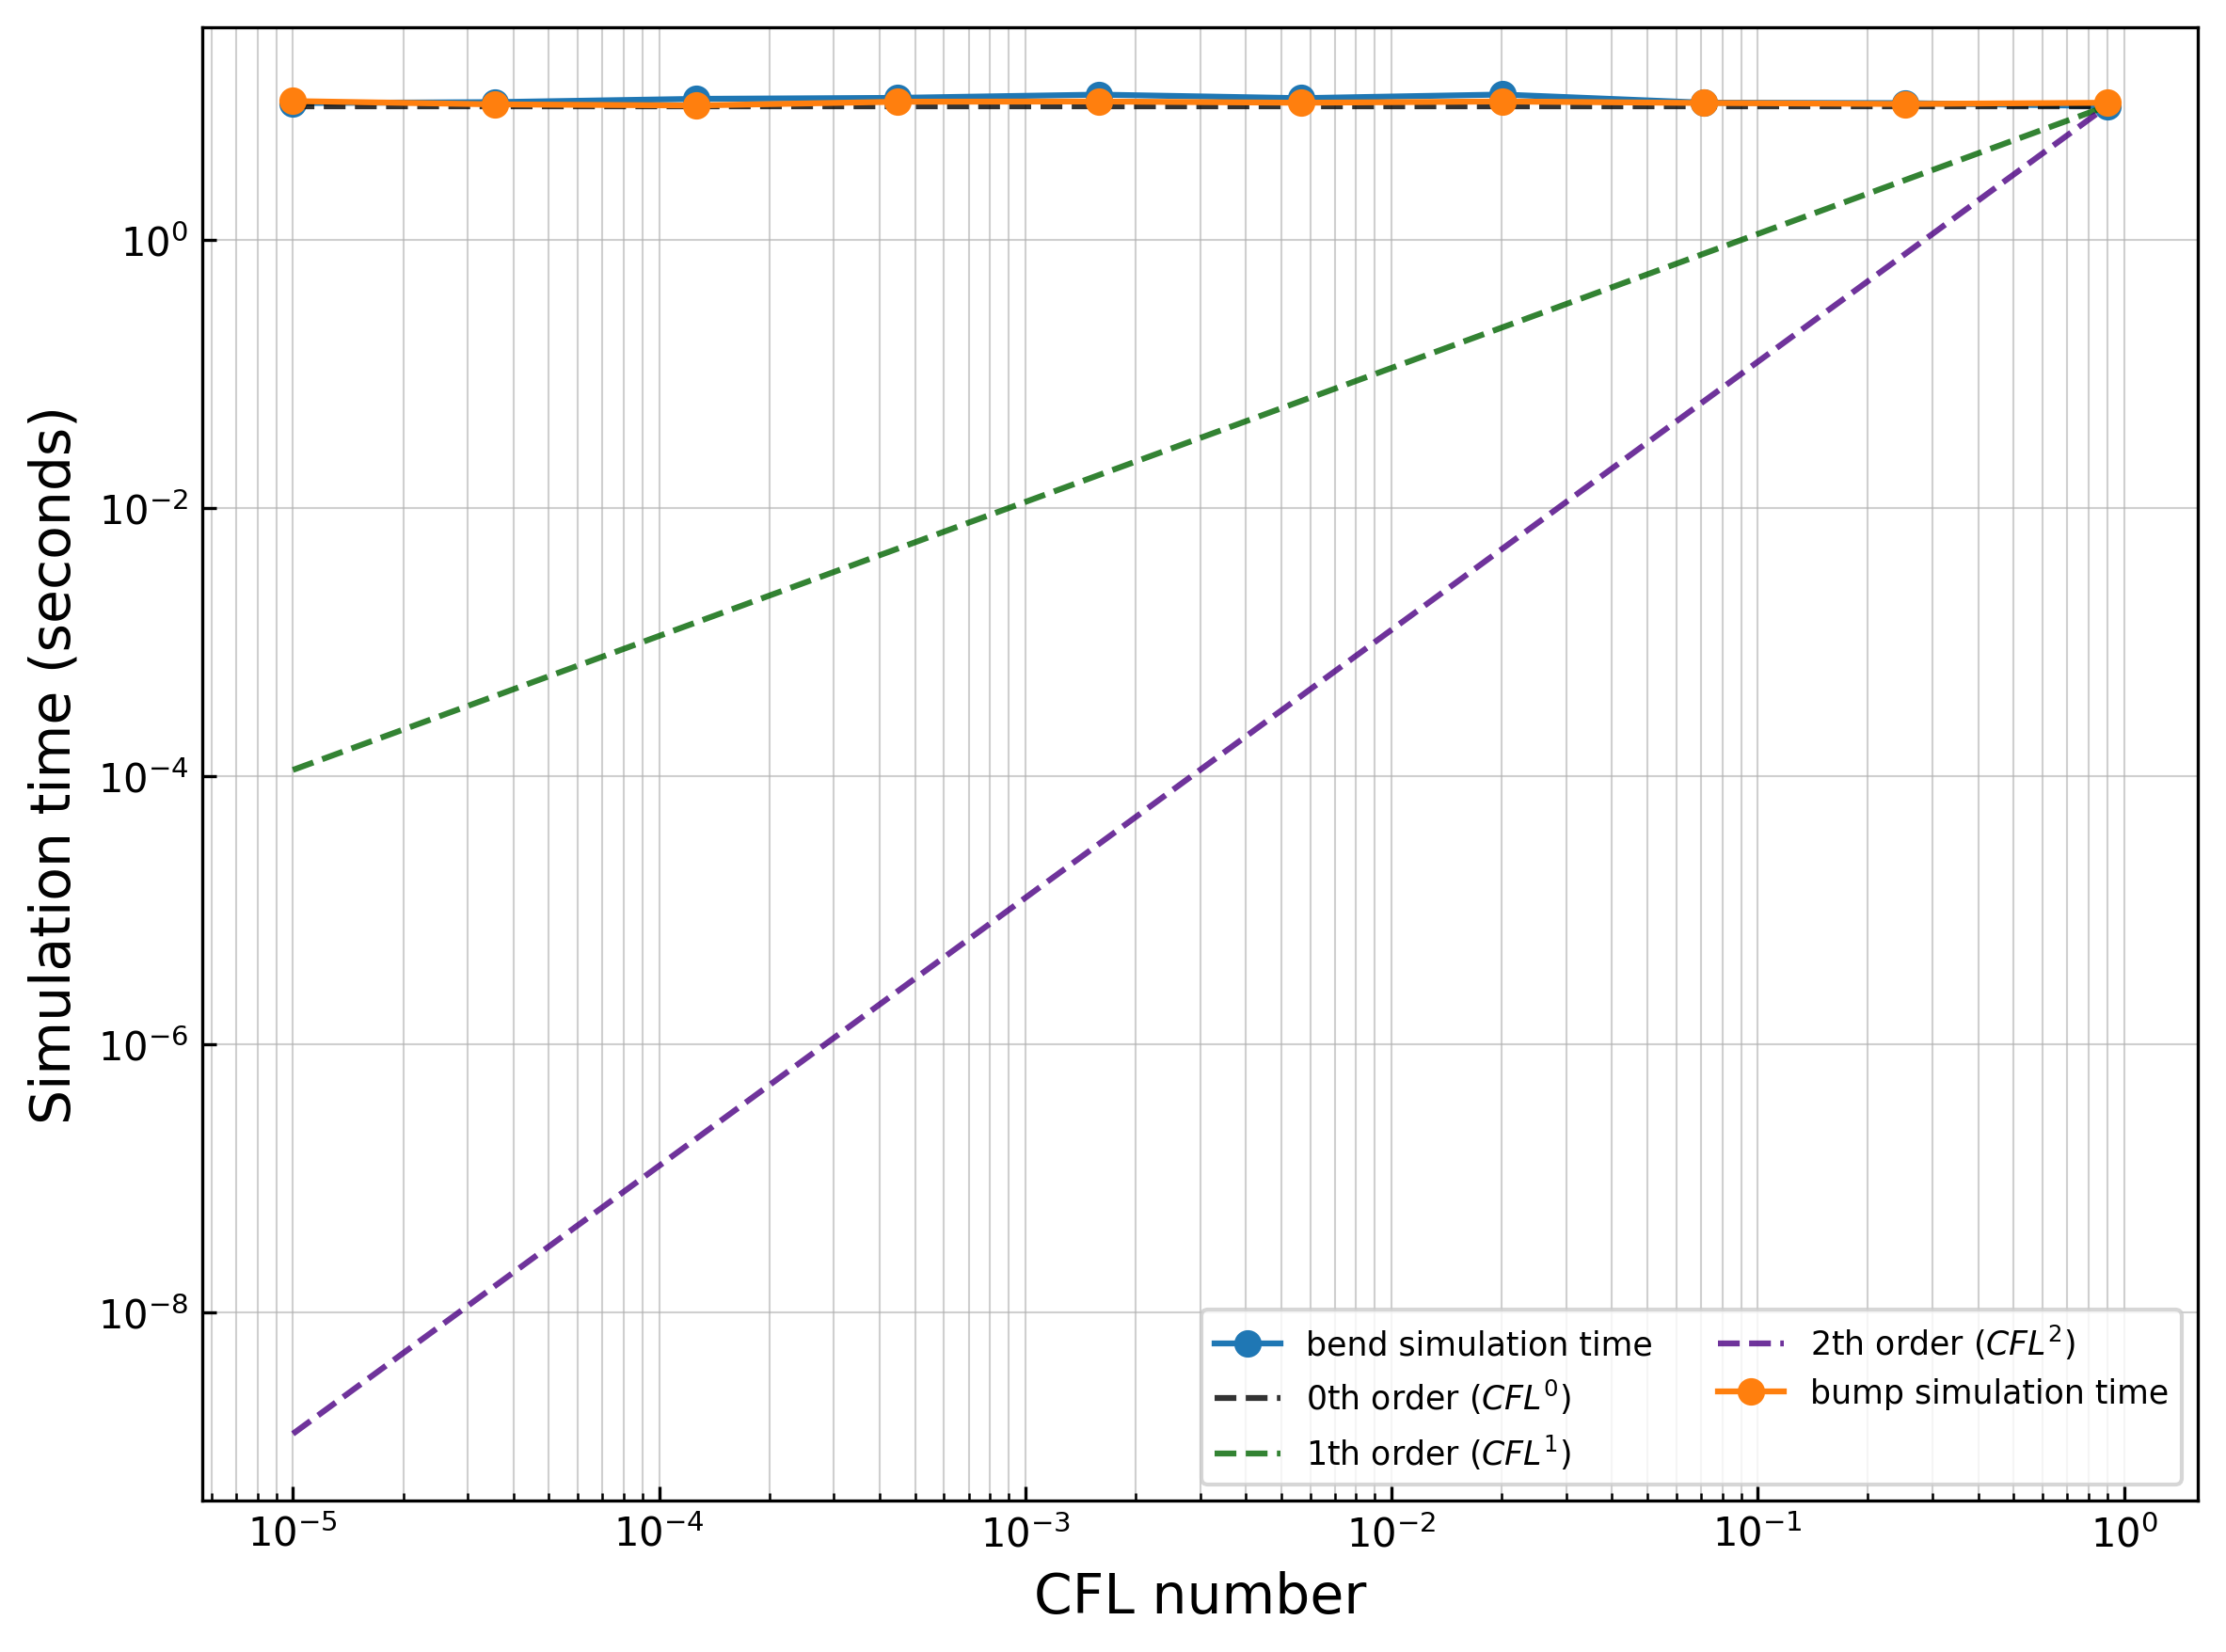
\includegraphics[width=\linewidth]{plots/simulation_time_bend_bump_CFL.png}
    \caption{Time results of the bend and bump cases with varying CFL numbers.}
    \label{fig:time_simulation_cfl}
\end{figure}

\subsection{Effects of varying smoothing factor}

\begin{figure}[H]
    \centering
    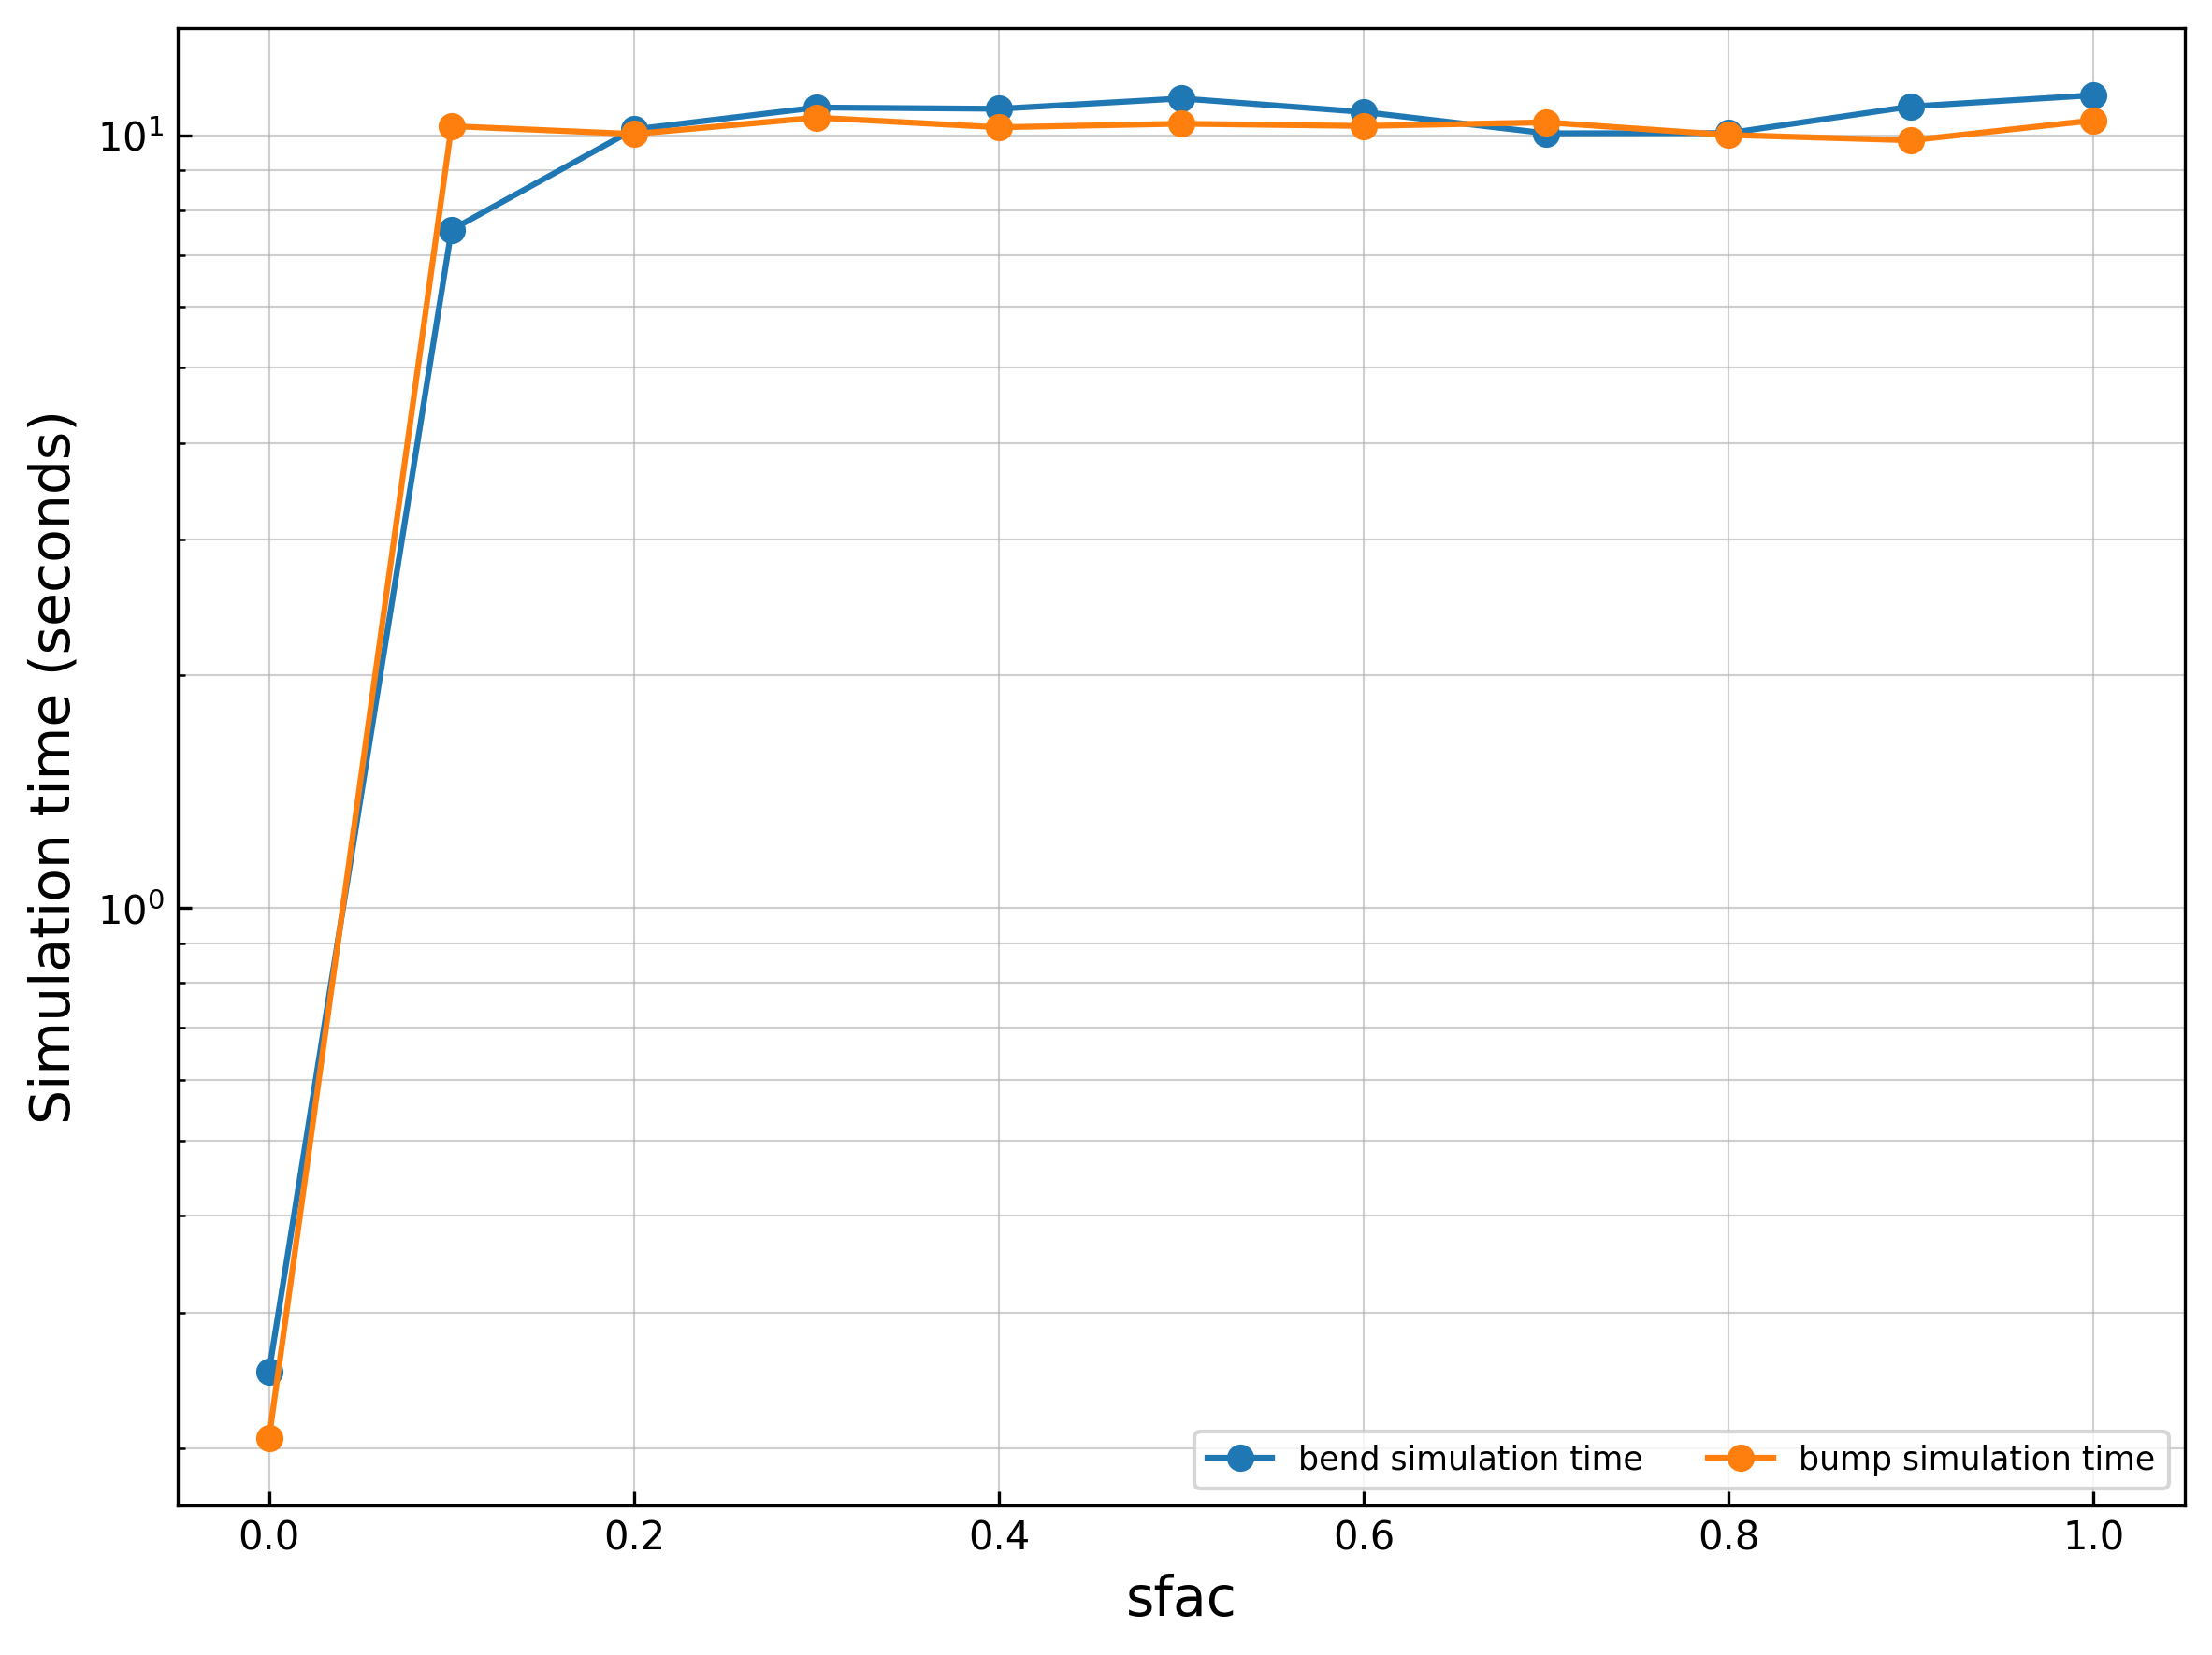
\includegraphics[width=\linewidth]{plots/simulation_time_bend_bump_sfac.png}
    \caption{Time results of the bend and bump cases with varying smoothing factors ($sfac$).}
    \label{fig:time_simulation_smoothing}
\end{figure}

\section{Conclusions}

\end{document}